
\chapter{\'Etude du corpus de son \textit{grafic}}
\label{chap:grafic}
Au chapitre précédent, le comportement de la NMF vis à vis des environnements sonores urbains était étudiée avec l'aide du corpus élémentaire \textit{Ambiance}. Le corpus était composé selon des niveaux sonores du trafic particulier avec des sources sonores spécifiques pris isolément. Dans ce chapitre, en vue de tester le comportement de la NMF sur des mixtures sonores plus proches d'enregistrements qui pourraient être réalisés en ville, celle-ci est maintenant appliquée sur le corpus élémentaire \textit{SOUR}.  
fait l'objet de test perceptif

qui étudié le comportement de la NMF , La combinaison de modalités qui obtiendra les erreurs les plus faibles pourra être considéré pour être intégré dans des capteurs embarqués?

\section{Rappel des facteurs expérimentaux}

Le corpus SOUR est composé de 74 fichiers audio d'une durée totale de 2h50, divisé en 4 ambiances sonores : \textit{Parc} (8 scènes), \textit{Rue calme} (35 scènes), \textit{Rue bruyante} (23 scènes), \textit{Rue très bruyante} (8 scènes). Le corpus est présenté en détail dans la partie \ref{part:corpus_grafic}.

L'estimateur \textit{baseline} reste le même que dans le chapitre \ref{chap:ambiance} : un filtre passe-bas de fréquence de coupure $f_c$ avec $f_c \in \lbrace 100,~500,~1k,~2k,~5k,~10k,~20k \rbrace$.
L'estimateur NMF est là encore basé sur la NMF supervisée (NMF SUP), semi-supervisée (NMF SEM) et seuillée initialisée (NMF IS). Le choix de la $\beta$-divergence se circonscrit à $\beta \in \lbrace 0,~1,~2 \rbrace$.
L'apprentissage du dictionnaire suit les même étapes que dans le chapitre précédent : chaque spectrogramme, issus des 53 fichiers audio constituant le corpus d'apprentissage, est découpé en trame temporelle de durée $w_t \in \lbrace 0,5,~1,~2 \rbrace$. Les valeurs \textit{rms} sont ensuite calculées selon la fréquence. L'algorithme de clustering $K$-mean est ensuite appliquée. Comme le corpus est plus petit, on étend le nombre d'éléments dans $\mathbf{W}$ à $K \in \lbrace 25,~50,~100,~200,~ 300 \rbrace$.
Pour la NMF SEM, le nombre d'élément dans le dictionnaire $\mathbf{W_r}$, pour le NMF SS, est maintenu à $J = 2$.
Dans le cas de la NMF IS, l'influence de l'opérateur sigmoïde dans le calcul de la distance et l'utilisation du seuil \textit{firm} s'étant relevés très faible, le choix a été fait de réduire l'étude au seul cas de représentation linéaire de la distante avec un seuillage dur afin de réduire les temps de calculs.
Comme les scènes sonores sont plus longues (de 1 min jusqu'à 3 minutes), le nombre d'itération est étendu à 400. 
Le résumé de ces paramètres se trouve dans le Tableau \ref{tab:experimental_factorsNMF}.
 

La durée des scènes dans le corpus SOUR n'étant pas la même, à l'inverse du corpus \textit{Ambiance}, c'est l'erreur $MAE$ toute les 60 secondes qui est calculée, $MAE_{60}$ afin d'avoir une durée normalisée : 

\begin{equation}
MAE_{60} = \frac{\sum_{1}^{M_60}\vert L_{eq,trafic,60s} - \tilde{L}_{eq,trafic,60s}\vert}{M_{60}}
\end{equation}

Pour cela, on calcule les niveaux sonores équivalent toutes les secondes. puis pour chaque ambiance, ces évolution sont cumulées. Puis, l'erreur est calculé en prenant en compte 60 secondes successivement. Ainsi il est possible de calculer une erreur dont une partie de l'erreur est calculé à partir d'une scène et l'autre partie de la scène suivante.

\begin{equation}
L_{eq,trafic,60s} = 10 \times \log_{10}\left(\frac{1}{60}\int_{t_{init}}^{t_{init}+60} 10^{L_{p,trafic,1s}(t)/10} dt\right)
\end{equation}

L'erreur $MAE_{60}$ pour chaque association de modalité est alors estimée. Puis l'erreur globale sur l'intégralité des ambiances sonores est calculé pour déterminer la combinaison de modalités de l'estimateur optimale sur l'ensemble du corpus :
  
\begin{equation}
MAE_{g} = \frac{\sum_{i = 1}^4 MAE_{60,i}}{4}.
\end{equation}

Le choix a été fait de ne pas pondérer l'erreur $MAE_{g}$ selon le nombre d'erreurs $MAE_{60}$ calculé par ambiance. Par leur durée plus importante, une moyenne pondérée serait plus influencée par les ambiances \textit{rue calme} et \textit{rue bruyante}. Afin de déterminer la combinaison la plus efficace sur l'ensemble des ambiances, le même poids est donc donné à chaque ambiance sonore.


\begin{table*}[t]
\centering
\caption{Facteurs expérimentaux et leur modalité utilisé pour le coprus SOUR.}
\begin{tabularx}{17.5cm}{L{3cm}@{}C{12cm}@{}C{2cm}@{}}
	\hline
    \textbf{\begin{tabular}[c]{@{}l@{}}facteur \\ expérimentaux \end{tabular}} & \textbf{modalités} & \begin{tabular}[c]{@{}C{2cm}@{}}\textbf{nombre de}\\ \textbf{modalité}\end{tabular}\\ \toprule
\end{tabularx}

\begin{tabularx}{17.5cm}{L{3cm}@{}C{3cm}@{}@{}C{3cm}@{}@{}C{3cm}@{}@{}C{3cm}@{}C{2cm}@{}}
    \textbf{Environnement sonore} & \begin{tabular}[c]{@{}c@{}}parc\\ 'Pa'\end{tabular} & \begin{tabular}[c]{@{}c@{}}rue calme \\ 'Ca'\end{tabular} & \begin{tabular}[c]{@{}c@{}}rue bruyante\\ 'Br' \end{tabular}& \begin{tabular}[c]{@{}c@{}}rue très bruyante\\ 'TrBr'\end{tabular} & 4\\
\end{tabularx}

\begin{tabularx}{17.5cm}{L{3cm}@{}C{3cm}@{}@{}C{3cm}@{}@{}C{3cm}@{}@{}C{3cm}@{}C{2cm}@{}}
	\rowcolor[HTML]{C0C0C0}
  \textbf{méthode} & filtre passe bas & NMF SUP & NMF SEM & NMF IS & 4\\
\end{tabularx}

\begin{tabularx}{17.5cm}{L{3cm}@{}@{}C{1.714cm}@{}@{}C{1.714cm}@{}@{}C{1.714cm}@{}@{}C{1.714cm}@{}@{}C{1.714cm}@{}@{}C{1.714cm}@{}@{}C{1.714cm}@{}C{2cm}@{}}
   $\mathbf{f_c}$ (kHz) & 1 & 0.5 & 1 & 2 &  5 & 10 & 20 & 7\\
\end{tabularx}

\begin{tabularx}{17.5cm}{L{3cm}@{}C{3cm}@{}@{}C{3cm}@{}@{}C{3cm}@{}@{}C{3cm}@{}C{2cm}@{}}
\rowcolor[HTML]{C0C0C0}
    $\mathbf{w_t}$ (s)& 0.5 & 1 & 2 & \textit{all} & 4\\
\end{tabularx}

\begin{tabularx}{17.5cm}{L{3cm}@{}C{2.4cm}@{}@{}C{2.4cm}@{}@{}C{2.4cm}@{}@{}C{2.4cm}@{}@{}C{2.4cm}@{}C{2cm}@{}}
    $\mathbf{K}$ & 25 & 50 & 100 & 200 & 300 & 5\\
\end{tabularx}

\begin{tabularx}{17.5cm}{L{3cm}@{}C{4cm}@{}@{}C{4cm}@{}@{}C{4cm}@{}C{2cm}@{}}
\rowcolor[HTML]{C0C0C0}
   $\mathbf{\beta}$ & 0 & 1 & 2 & 3\\
\end{tabularx}

\begin{tabularx}{17.5cm}{L{3cm}@{}C{12cm}@{}C{2cm}@{}}
   seuillage dur $\mathbf{t_h}$ & de 0.20 à 0.60 avec un pas de 0.01 & 41\\
   \bottomrule
\end{tabularx}
\label{tab:experimental_factorsNMF}
\end{table*}

\section{Résultats des estimateurs}

\subsection{Erreurs produites par l'estimateur \textit{baseline}}
Dans un premier temps, les erreurs réalisées par la baseline sont observés sur l'ensemble du corpus et selon chaque ambiance (Tableau \ref{tab:grafic_baseline}).

\begin{table}[h]
\caption{Erreurs moyennes $MAE_{g}$ et $MAE_{60}$ pour l'estimateur \textit{baseline}.}
\label{tab:grafic_baseline}
\centering
\begin{tabular}{L{1.6cm}C{2.5cm}@{}@{}C{2.1cm}@{}@{}C{2.1cm}@{}@{}C{2.1cm}@{}@{}C{2.2cm}@{}@{}}
\toprule
$f_c$ (Hz) & $MAE_{g}$ & $MAE_{60,Pa}$ & $MAE_{60,Ca}$ & $MAE_{60,Br}$  & $MAE_{60,TrBr}$ \\
\midrule
100 & 2,93 ($\pm$ 0,60) & \textbf{2,53} & 3,98 & 2,69 & 2,69 \\
500 & \textbf{\textcolor{red}{2,03 ($\pm$ 1,43)}} & 4,00 & \textbf{2,18} & 0,93 & 1,03 \\
1k & 2,45 ($\pm$ 2,62) & 6,17 & 2,48 & \textbf{0,63} & 0,58 \\
2k & 3,00 ($\pm$ 3,32) & 7,69 & 2,98 & 0,95 & \textbf{0,38} \\
5k & 3,50 ($\pm$ 3,90) & 9,01 & 3,44 & 1,13 & 0,42 \\
10k & 3,61 ($\pm$ 3,99) & 9,24 & 3,61 & 1,17 & 0,43 \\
20k & 3,64 ($\pm$ 4,00) & 9,28 & 3,65 & 1,20 & 0,44 \\
\bottomrule         
\end{tabular}
\end{table}

Là encore, c'est le filtre passe-bas à la fréaquence de coupure $f_c$ = 500 Hz qui offre l'erreur $MAE_g$ la plus faible ($MAE_g$ = 2,03 ($\pm$ 1,43)).  En détaillant selon chaque ambiance, on retrouve un comportement similaire à celui observé pour le corpus \textit{ambiance} : plus la part de la source \textit{trafic} est présente plus la fréquence de coupure, correspondant à la plus faible erreur, augmente. Une fois encore, l'estimateur filtre Passe-Bas pour $f_c$ = 500 Hz revient à un compromis entre les différentes ambiances selon l'énergie rejeté et l'énergie conservée.
On remarque enfin que l'erreur à 20 kHz excède 3 dB qui correspond à la valeur d'incertitude acceptée lors des estimations des niveaux de bruits.

\subsection{Erreurs produites par l'estimateur NMF}
\label{chap:grafic_nmf}

Les erreurs générées par l'estimateur NMF selon les multiples associations des modalités des facteurs expérimentaux sont ensuite détaillés. Ayant, là encore, un nombre important de résultat, on ne détaille ici que les résultats les plus performants selon chaque méthode et valeur de $\beta$. La composition du corpus \textit{SOUR} étant différente de celle du corpus \textit{Ambiance}, les combinaisons optimales différents dans certains cas. 

\begin{table}[h]
\centering
\caption{Erreurs $MAE_{60}$ pour les combinaisons optimales de modalités des estimateurs pour le corpus d'évaluation SOUR.}
\label{tab:erreur_mae60}
\begin{tabular}{L{2cm}C{1.2cm}C{1.2cm}C{1.2cm}C{1.2cm}C{1.2cm}C{2.5cm}C{2.5cm}}
\toprule
méthode & $f_c$ (kHz) & $\beta$ & $w_t$ & K & $t_h$ & $MAE_{60}$ \\ \toprule
\multirow{2}{*}{filtre PB} & 20 & - & - & - & - &  3,64 ($\pm$ 4,00) \\
 & 0,5 & - & - & - & - & 2,03 ($\pm$ 1,43) \\ \midrule
\multirow{3}{*}{NMF SUP} & - & 0 & 0,5 & 200 & - & 4,01 ($\pm$ 4,43) \\
 & - & 1 & 2 & 25 & - & 2,69 ($\pm$ 2,90) \\
 & - & 2 & 0,5 & 25 & - & 2,22 ($\pm$ 2,33) \\ \midrule
\multirow{3}{*}{NMF SEM} & - & 0 & 2 & 300 & - & 2,13 ($\pm$ 0,63) \\
 & - & 1 & 2 & 300 & - & 1,98 ($\pm$ 0,59) \\
 & - & 2 & 2 & 300 & - & 2,23 ($\pm$ 1,41) \\ \midrule
\multirow{3}{*}{NMF IS} & - & 0 & 1 & 25 & 0,32 & 1,43 ($\pm$ 0,73) \\
 & - & 1 & \textit{all} & 50 & 0,34 &  1,32 ($\pm$ 1,15) \\
 & - & \textbf{2} & \textbf{1} & \textbf{300} & \textbf{0,35} & \textbf{\textcolor{red}{1,20 ($\pm$ 0,87)}} \\
 \bottomrule
\end{tabular}
\end{table}

La NMF SUP se révèle pour ce corpus moins bonne que l'estimateur \textit{baseline} à $f_c$ = 500 Hz avec des écart-types plus importants notamment pour l'estimateur basé sur la divergence d'Itakura-Saïto ($\beta$ = 0). 2 méthodes privilégient un faible nombre d'élément dans le dictionnaire ($K$ = 25) à l'exception de celle basé sur la divergence d'Itakura Saïto. 

Les version optimales de la NMF SEM sont basées sur le même dictionnaire et privilégient un grand nombre d'éléments dans le dictionnaire ($K$ = 300). Leur erreurs ne diffèrent donc que par le choix de $\beta$. Si la NMF SEM propose des erreurs plus faibles que la NMF SUP, elle n'améliore les performances de l'estimateur \textit{baseline} que pour $\beta$ = 1.  
Enfin, la NMF IS qui se révèle être les plus performantes avec systématiquement des erreurs inférieures à 1,5. La méthode la plus performante est celle basée sur la distance euclidienne avec $K$ = 300, $w_t$ = 1 s et un seuil $t_h$ = 0,35. On constate que pour $\beta \in \lbrace 0,~1 \rbrace$, à l'inverse du corpus \textit{Ambiance}, le nombre d'éléments est ici réduit, respectivement à 25 et 50.
Les valeurs seuils sont plus faible que pour ce corpus puisque la part du trafic est ici plus importante que dans le corpus \textit{Ambiance}. Afin d'inclure les éléments \textit{trafic}, 

Les classes de sons dans le corpus appartiennent majoritairement aux classes interférantes \textit{alerte}, \textit{animaux} et \textit{humains}, des classes de sons dont les spectres sont moins similaires à ceux du trafic. Conséquence, la $D_{\theta}$ entre les éléments \textit{trafic} et ceux modélisant ces sources est plus faible. Donc en diminuant le seuil, on arrive à toujours mettre à part les classes interférantes et à conserver plus d'éléments dans $\mathbf{W}_{trafic}$. 

\begin{figure}[h]
\centering
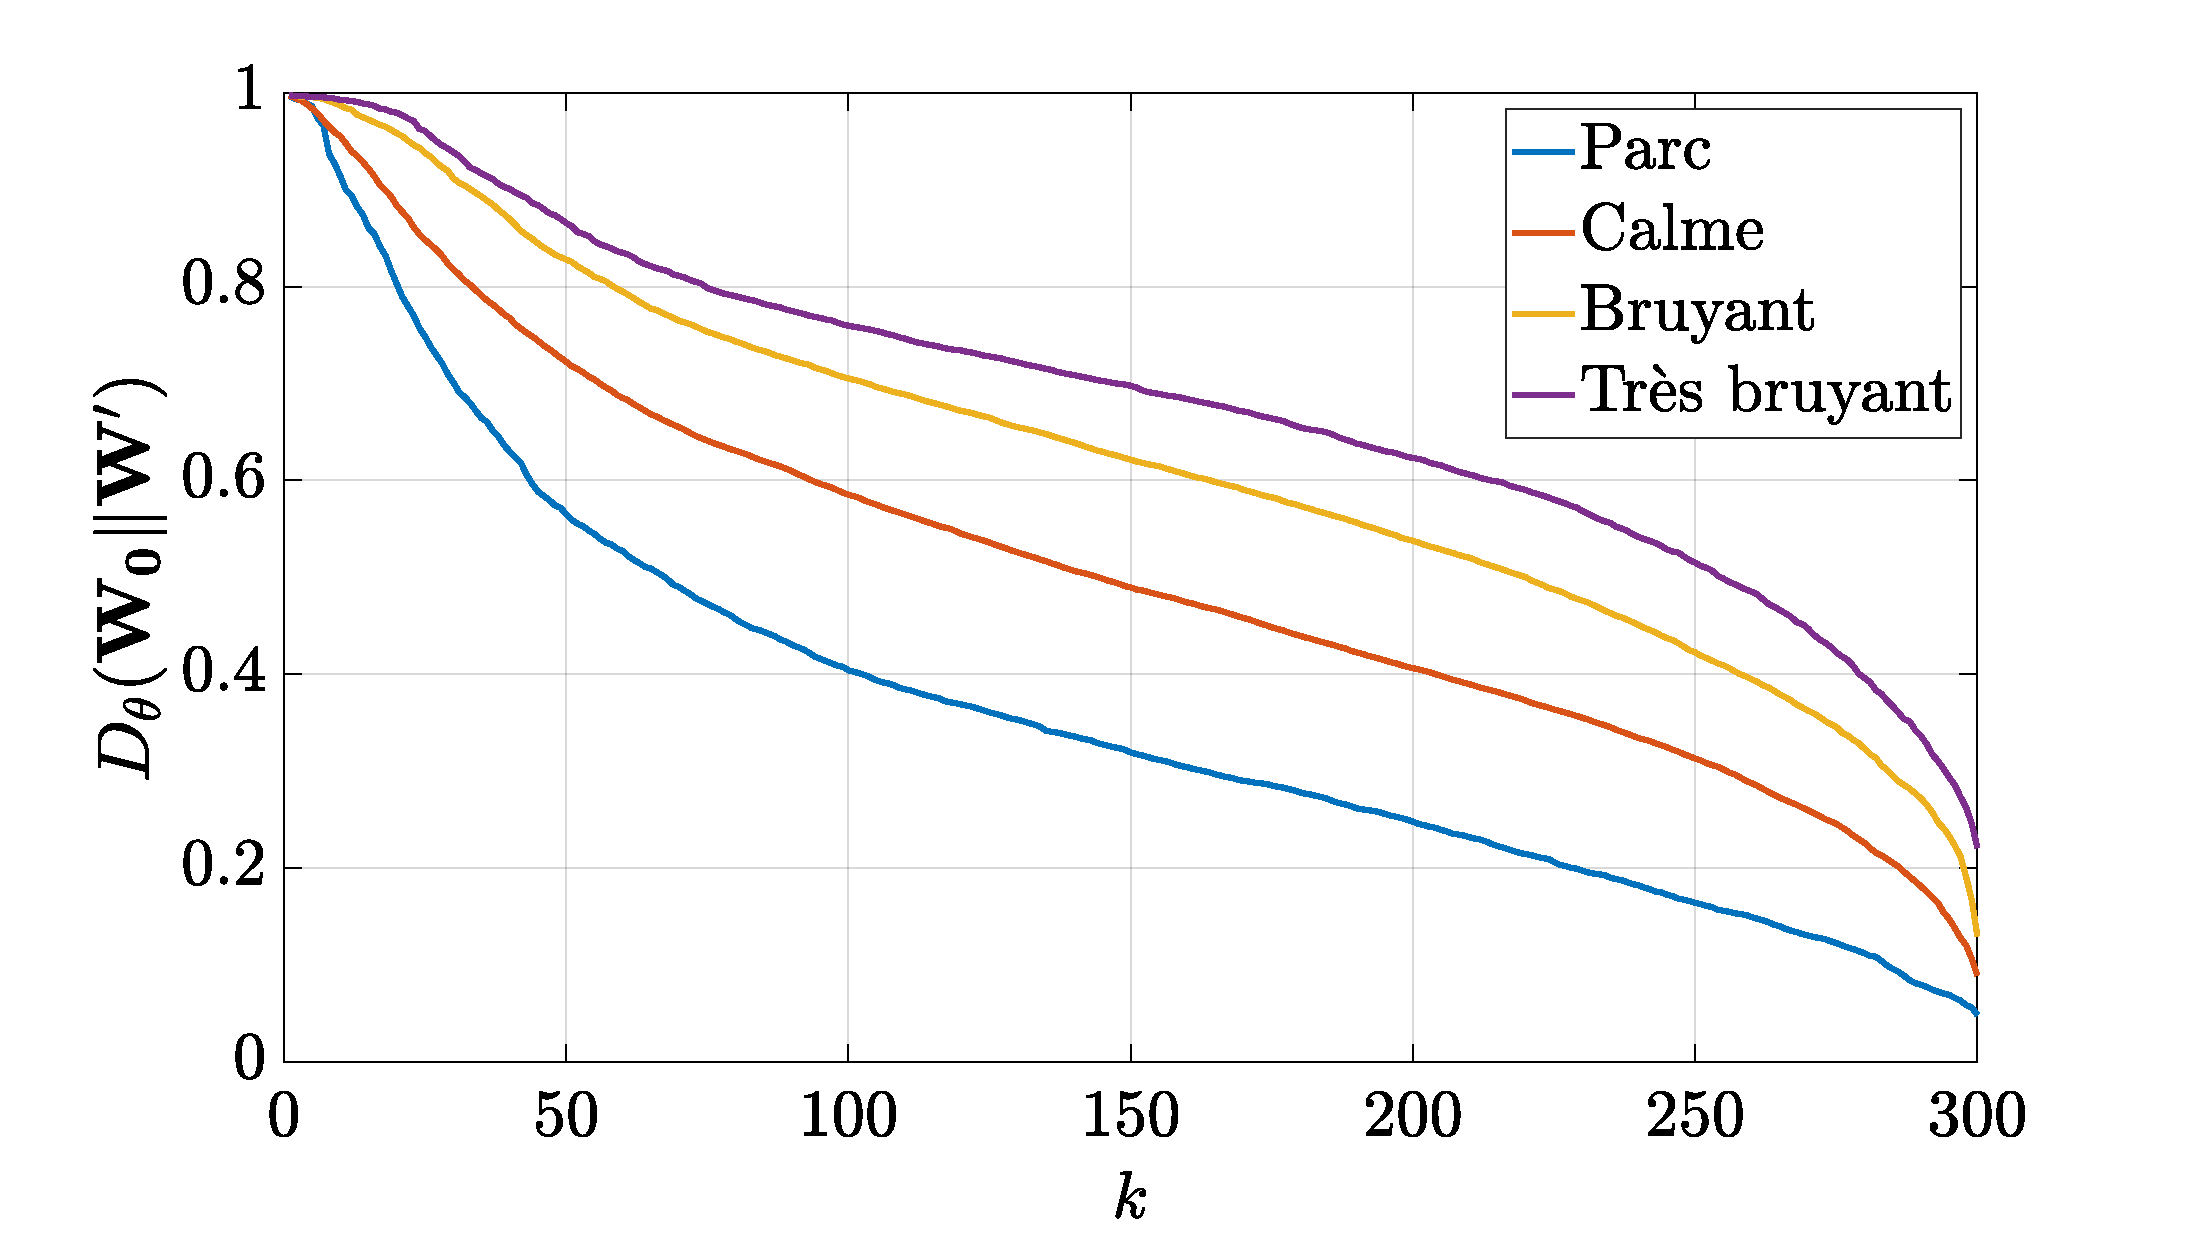
\includegraphics[width=.7\linewidth]{./figures/resultats/dist_grafic.pdf}
\caption{Distances $D(\mathbf{W_0}\Vert \mathbf{W'})$ moyennes par ambiance sonore triées par ordre décroissant.}
\label{fig:dist_grafic}
\end{figure}

L'erreur par ambiance sonore est ensuite détaillée selon les combinaisons optimales de chaque méthode. Le temps de calcul mis par l'estimateur pour extraire la composante \textit{trafic} d'un spectrogramme $\mathbf{V}$ d'uen durée de 1 minute est ajouté. Dans le cas de la NMF, c'est le temps mis par la méthode pour réaliser les 400 itérations.

\begin{table}[h]
\centering
\caption{Erreurs $MAE_{60}$ selon les estimateurs NMF pour chaque méthode dans sa combinaison optimale de modalités avec les estimateurs \textit{baseline} à 500 Hz et 20 kHz.}
\label{tab:erreur_mae60_amb}
\resizebox{\textwidth}{!}{%
\begin{tabular}{L{4cm}C{2.5cm}C{2.5cm}C{2.5cm}C{2.5cm}C{2.5cm}}
\toprule
méthode & Parc & Rue Calme & Rue Bruyante & Rue très bruyante & temps de calcul/min (s)\\ \midrule
filtre PB, $f_c$ = 20 kHz & 9,97 ($\pm$ 5,08) & 3,54 ($\pm$ 2,25) & 1,08 ($\pm$ 0,53)& 0,45 ($\pm$ 0,38)&  0,03 ($\pm$ 0,01) \\
filtre PB, $f_c$ = 500 Hz & 4,80 ($\pm$ 5,08) & 1,87 ($\pm$ 2,25) & 0,92 ($\pm$ 0,54) & 0,96 ($\pm$ 0,38) &  0,03 ($\pm$ 0,01) \\ \midrule
NMF SUP & 5,58 ($\pm$ 5,06)  & 2,00 ($\pm$ 2,22) & 0,66 ($\pm$ 0,56) & 0,64 ($\pm$ 0,33) & 0,19 ($\pm$ 0,03)\\
NMF SEM & 2,69 ($\pm$ 2,71) & 2,36 ($\pm$ 2,42) & 1,58 ($\pm$ 0,87) & 1,38 ($\pm$ 0,60) & 3,55 ($\pm$ 0,13)\\
NMF IS & \textbf{\textcolor{red}{2,21 ($\pm$ 3,84)}} & \textbf{\textcolor{red}{1,64 ($\pm$ 1,85)}} & \textbf{\textcolor{red}{0,61 ($\pm$ 0,54)}} &  \textbf{\textcolor{red}{0,34 ($\pm$ 0,20)}} & 4,30 ($\pm$ 0,31)\\ \bottomrule
\end{tabular}}
\end{table}

La NMF IS se révèle la méthode la plus performante pour 3 ambiances sonores. La NMF SEM propose la plus faible erreur pour les ambiances \textit{Parc} qui correspondent aux scènes où le trafic est le moins présent. 
La NMF SUP conserve son comportement : peu efficace pour les scènes sans trafic et meilleure lorsque le trafic devient prédominant. Seulement ici, la NMF IS est meilleure !

On trace l'évolution de l'erreur $MAE_{60}$ selon le nombre d'éléments dans $\mathbf{W}$ pour la NMF IS dans sa combinaison optimale. On étend pour ce cas la dimension du dictionnaire jusqu'à 400 éléments. En parallèle de cette évolution le temps de calcul est adjoint. Il permet de constater l'influence du nombre d'éléments dans la NMF IS : l'erreur décroit avec l'augmentation de $\mathbf{K}$. Plus d'éléments dans le dictionnaire implique d'avoir plus de spectre et ainsi de mieux modéliser les variations de la source sonore. Cependant, cette diminution se fait au dépend du temps de calcul : celui-ci croit avec l'augmentation du rang du dictionnaire. Si entre $K$ = 25 et $K$ = 200, l'erreur chute significativement, à partir de $K$= 300 la diminution de l'erreur devient faible, la variation de l'erreur devient faible au regard de la variation du temps de calcul. Suivant les applications souhaités, il peut ne pas être judicieux d'augmenter la taille du dictionnaire.

\begin{figure}[h]
\centering
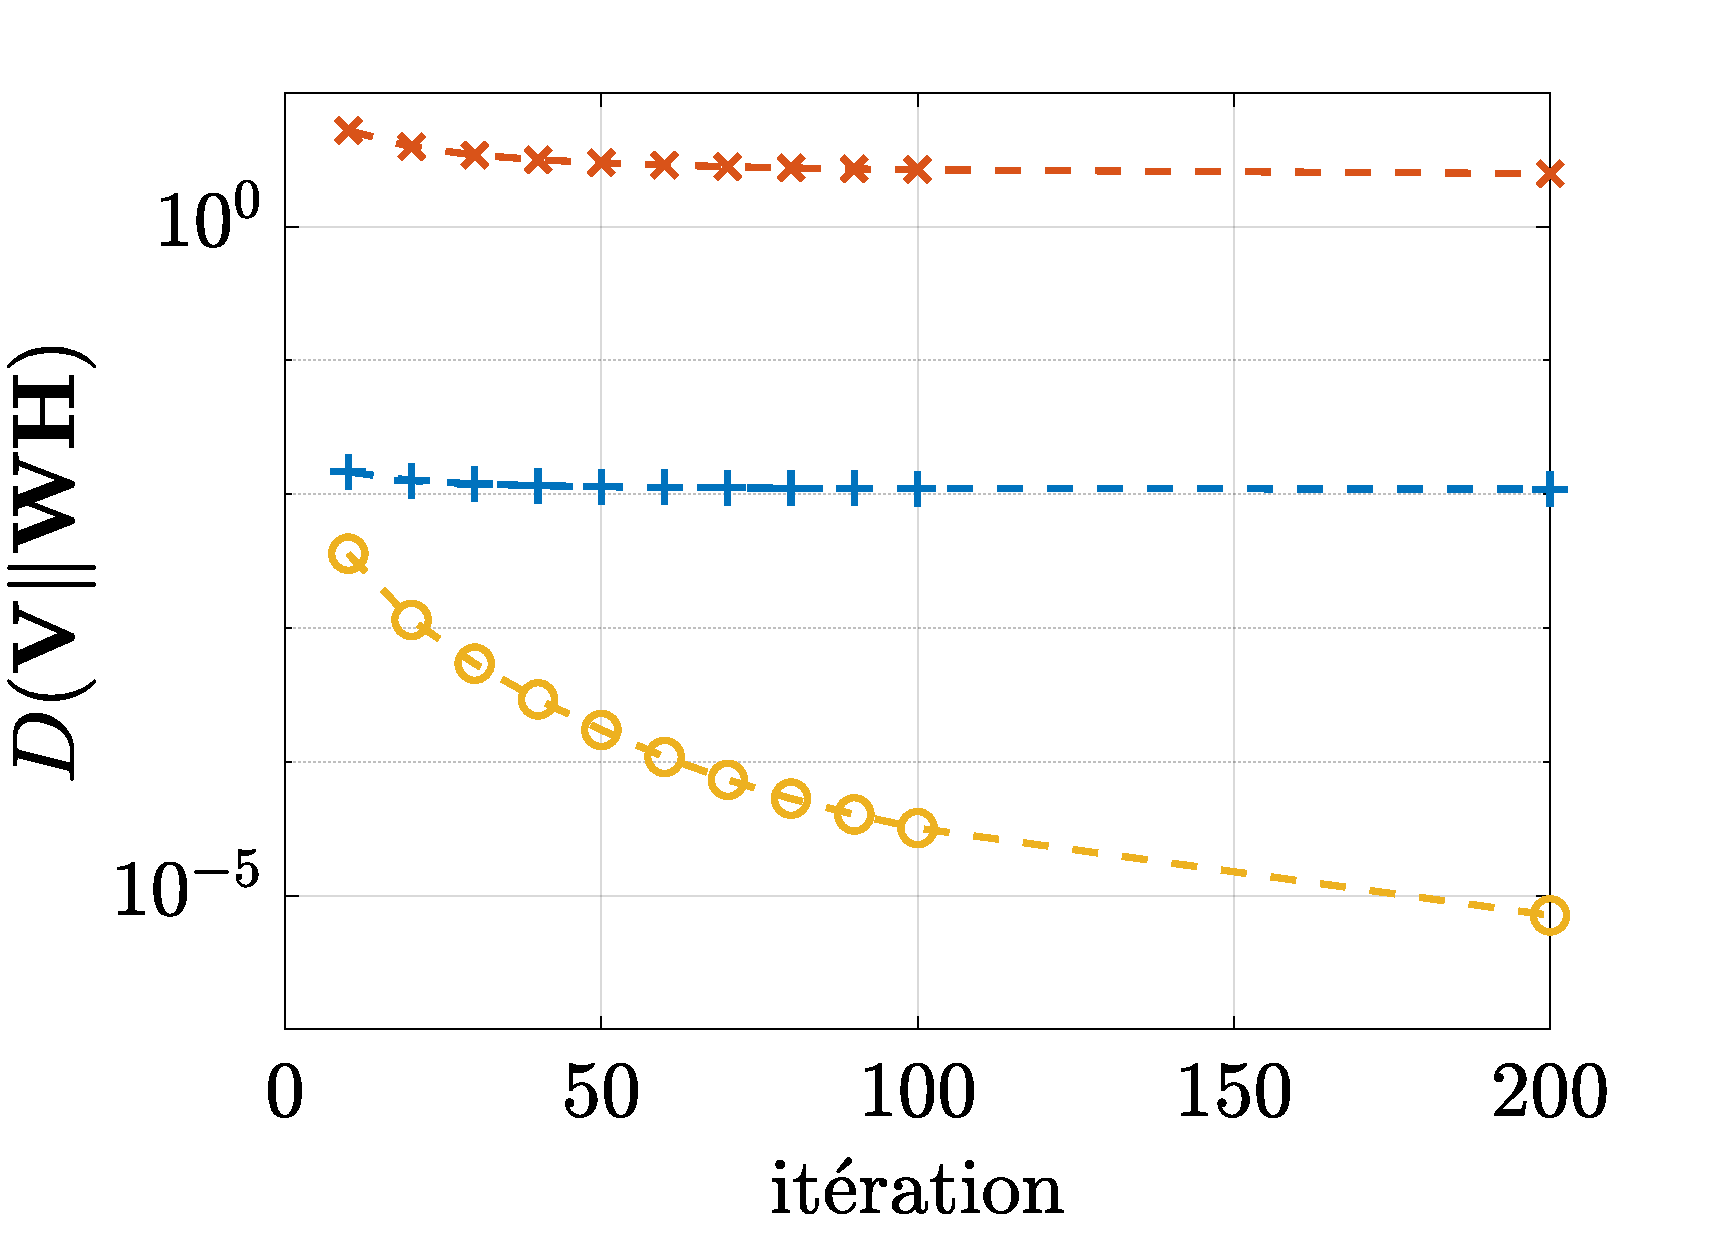
\includegraphics[width=.8\linewidth]{./figures/resultats/grafic_cost.pdf}
\caption{Fonction de coût moyen pour le corpus élémentaire SOUR selon les 3 NMF pour leur combinaison de facteurs optimale}
\end{figure}


La convergence de la NMF IS est meilleure sur l'ensemble des cas, la SEM est la moins efficace y compris sur l'ambiance \textit{parc} alors qu'elle y obtient la plus faible erreur. La NMF SUP et SEM sont rapidement constante, la mise à jour des matrices ne permettent pas d'améliorer la reconstruction de $\mathbf{V}$, la NMF IS, en mettant à jour $\mathbf{W}$ et $\mathbf{H}$ permet d'améliorer progressivement la reconstruction. En définitive, améliorant la reconstruction globale, elle arrive à en obtenir une meilleure du signal \textit{trafic}.



\begin{itemize}
\item résultats
\begin{itemize}
\item allure des courbes Lp,1s pour chaque ambiance

\item smoothness VVV et impact notable sur le semi-supervisée
\item optimisation de la valeur seuil en fonction d'indicateur
calibration qui fait défaut donc les valeurs de référence sont à revoir mais ça signifie qu'avec des indicateurs assez simple, on peut ajuster les seuils et optimiser tout cela !.
\end{itemize}
\end{itemize}




\subsection{Contrainte de régularité temporelle}
Afin de tenter d'améliorer ces résultats, une première contrainte est ajoutée sur la NMF par la contrainte de régularité temporelle. 

\begin{equation}
D(\mathbf{V}\Vert \mathbf{WH}) + \alpha C(H)
\end{equation}

Cette contrainte, présentée dans la partie \ref{} consiste à forcer les activateurs temporelles à adopter des variations plus lentes entre les trames temporelles. L'utilisation de cete contrainte est justifié ici par le comportement de la source d'intérêt : le passage d'une voiture est un évènement qui a une durée de plusieurs secondes. En forcant les activateurs à adopter des variations plus lentes, on serait à même de pouvoir mieux modéliser cette source. 

Dans les cas de la NMF SUP et le NMF IS, cette contrainte s'applique sur l'ensemble des matrices $\mathbf{H}$. Dans le cas de la NMF SEM, le dictionnaire se décompose en deux parties (une partie fixe $\mathbf{W_s}$ composée de spectres \textit{trafic} et d'une partie mobile $\mathbf{W_r}$). Pour favoriser les variations lentes des activateurs temporelles des spectres \textit{trafic}, cette contrainte est donc seulement posée pour $\mathbf{H_s}$. La mise à jour de la matrice suit donc celle de l'équation \ref{}. La mise à jour de $\mathbf{H_r}$ reste la même (équation \ref{eq:}).
Les valeurs de la pondération $\alpha$ permettent alors de contrôler l'influence de la contrainte. Elle est définit pour plusieurs valeurs : $\alpha = \lbrace$ 
contrainte sur Ws et pas sur Wr
faire K = 300 pour beta = 1 pour la TI NMF

\begin{table}[h]
\centering
\caption{Erreurs $MAE_{60}$ pour chaque estimateur NMF avec la contrainte de régularité.}
\label{tab:erreur_smooth}
\begin{tabular}{L{2cm}C{1.2cm}C{1.2cm}C{1.2cm}C{1.2cm}C{1.2cm}C{2.5cm}}
\toprule
 & $\beta$ & $K$ & $w_t$ & $t_h$ & $\alpha$ & $MAE_{60}$ \\ \midrule
\multirow{2}{*}{NMF SUP} & 2 & 25 & 0,5 & - & 0 & 2,22 ($\pm$ 2,33) \\
 & 2 & 25 & 0,5 & - & 0,01 & \textbf{2,13 ($\pm$ 2,20)} \\\midrule
\multirow{3}{*}{NMF SEM} & 1 & 300 & 2 & - & 0 & 1,98 ($\pm$ 0,51) \\
 & 1 & 300 & 2 & - & 0,10 & 1,87 ($\pm$ 0,41) \\
 & 0 & 300 & 2 & - & 0,50 & \textbf{1,55 ($\pm$ 0,98)} \\\midrule
\multicolumn{1}{c}{\multirow{2}{*}{NMF IS}} & \textbf{2} & \textbf{300} & \textbf{1} & \textbf{0,35} & \textbf{0} & \textbf{\textcolor{red}{1,20 ($\pm$ 0,87)}} \\
\multicolumn{1}{c}{} & 1 & 200 & 1 & 0,36 & 0,15 & 1,47 ($\pm$ 0,86)\\ \bottomrule
\end{tabular}
\end{table}


\begin{figure}[h!]
\centering
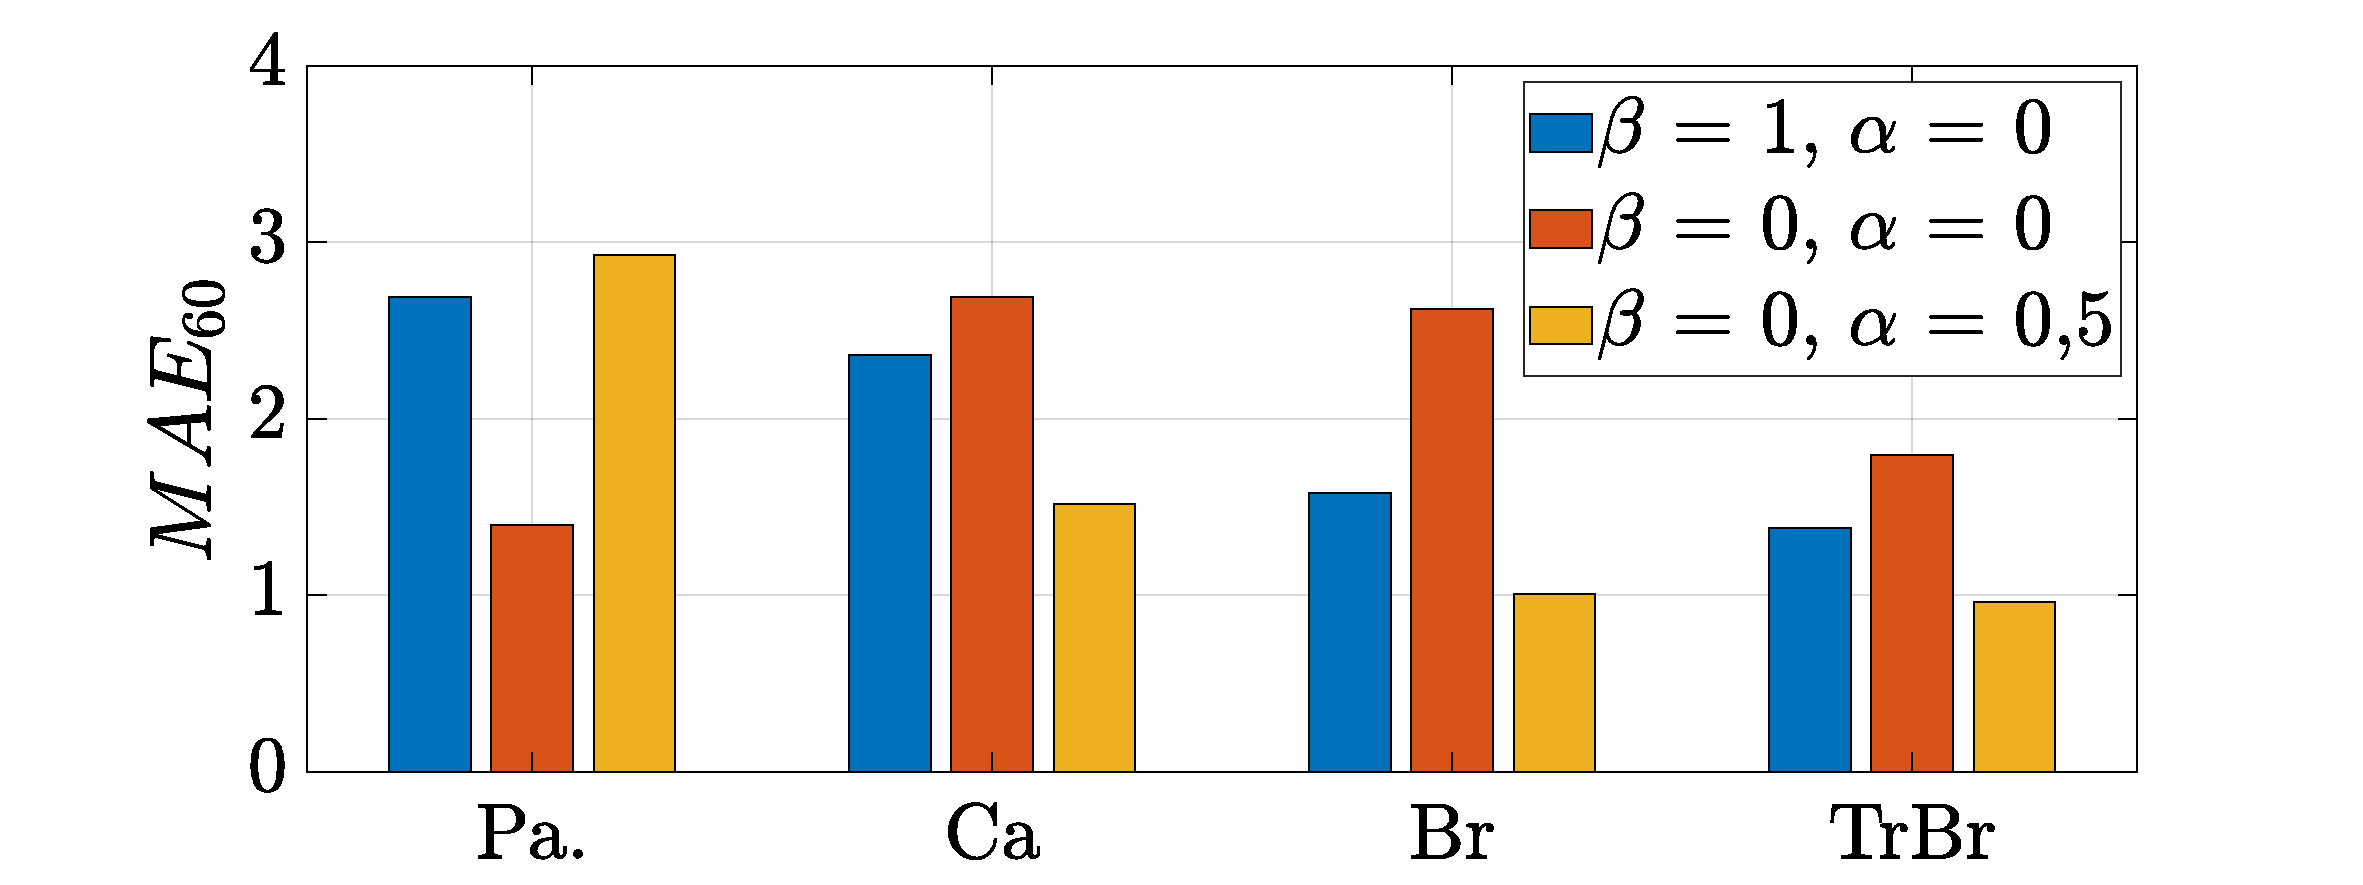
\includegraphics[width=.9\linewidth]{./figures/resultats/grafic_smooth_bar.pdf}
\caption{Influence de la pondération de régularité temporelle pour la NMF SEM selon chaque ambiance sonore.}
\end{figure}

\begin{figure}[h]
\centering
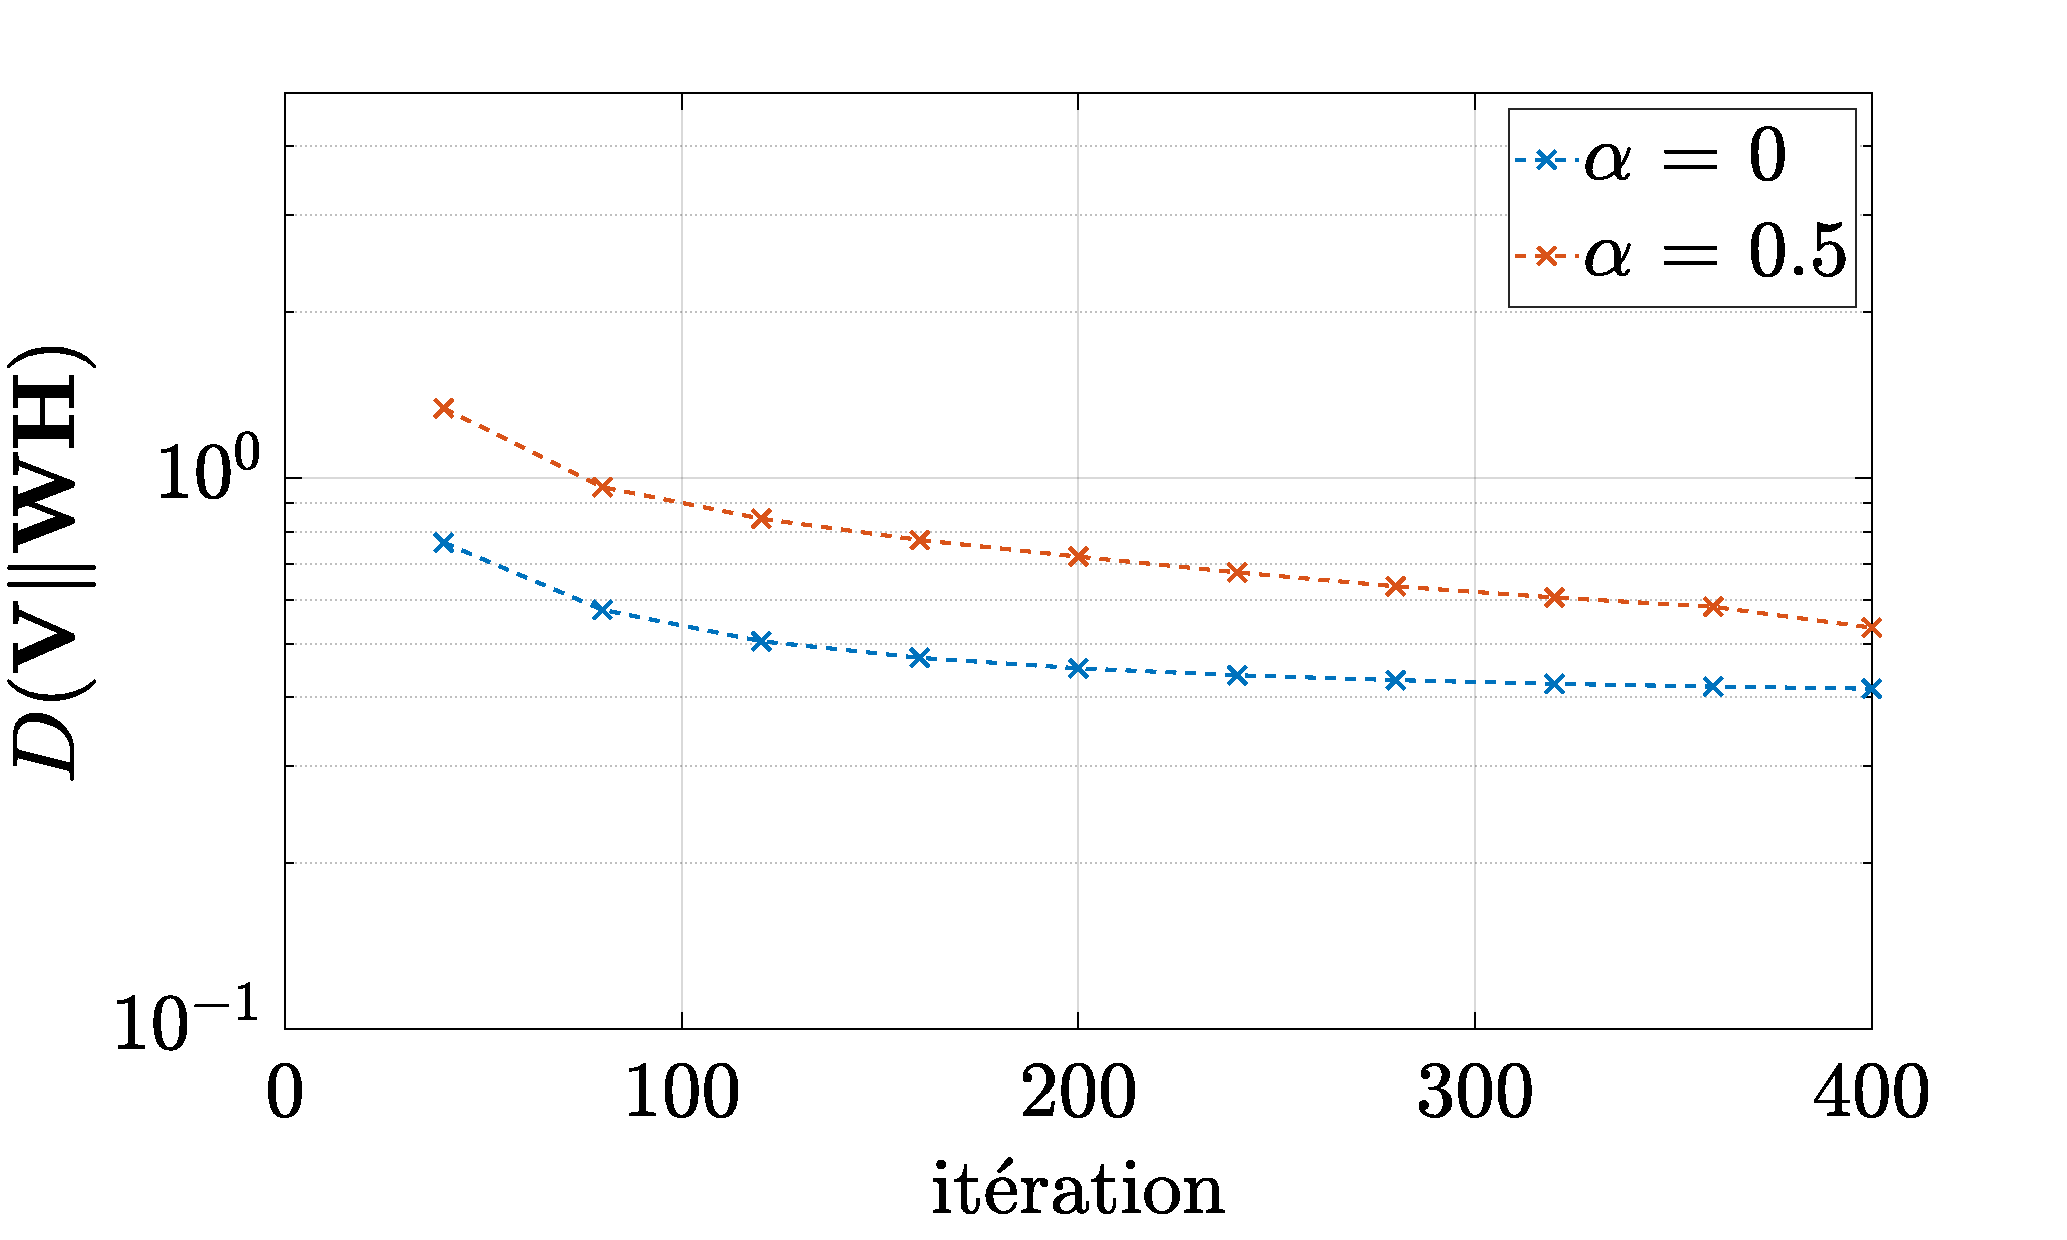
\includegraphics[width=.8\linewidth]{./figures/resultats/grafic_smooth_cost_beta0.pdf}
\caption{Influence de la régularité temporelle sur la fonction de coût.}
\end{figure}


\subsection{Contrainte par parcimonie}



\subsection{Optimisation par les seuils}


%On a déterminé un seuil optimal par ambiance :
%parc => th = 
%calme => th = 
%br => th = 
%tr_br=> th = 

Le but est de trouver des indicateurs simples qui serait corrélé à ces seuils


%\end{document}